%!TEX root = ../swiatlow_thesis.tex
\label{chapter:susy}

\section{The Problem of the Standard Model}
\label{chapter:susy:problems}

It is somewhat incongruous to say that the SM has problems after describing the huge degree of its success in Chapter~\ref{chapter:sm}, but there are clear tensions in the model which point to signs of potential new extensions. The following sections describe some of these shortcomings.

\subsection{The Pursuit of Beauty, or Naturalness}

The process of developing a fundamental theory of nature is intended to be simplifying: for example, the development of the parton model and QCD simplified the eight-fold way and the complicated sea of hadrons  that came before it. The core of this simplification was the realization of a symmetry-- the $SU(3)$ of color-- which reduced a complicated system to a more simple one. There is an element to this that a physicist might call beautiful: the realization of an underlying simple pattern which explains something complicated. In that sense, there should be very few accidents in a theory: there should be a \textit{reason} for things to be the way they are. For example, there are no accidental, or ad-hoc terms in a Lagrangian: we include all relevant terms allowed by the symmetry groups, and derive the consequences. The symmetry groups are the reason that the Lagrangians look the way they do.

In this same sense, constants in the theory can be arbitrary, but requiring them to be \textit{arbitrarily precise} is something of an aesthetic problem: the theory should not care if the mass of the up or down quark were different by $50\%$, for example. However, there is exactly one such finely tuned mass in the Standard Model-- $m_h$, the mass of the Higgs boson. 

As discussed in Section~\ref{chapter:sm:qcd:freedom}, higher-order terms caused by loop diagrams induce corrections to constants, such as masses and coupling constants, through the process of renormalization. The Higgs boson's mass is not immune, and since the Higgs couples to all particles (except gluons) via either electroweak symmetry breaking terms or the Yukawa couplings to matter, in principle all of these particles can create loops which correct the Higgs mass. Because it has the largest coupling, the loop involving the top quark-- pictured in Figure~\ref{fig:susy:higgs-loop}--  has the largest contribution out of all these terms. \editnote{cite Martin} The correction, in fact, goes as:
%
\begin{equation}
\Delta m_H^2 = - \frac{|y_T|^2}{8\pi^2}\Lambda_\mathrm{UV}^2 + \ldots
\end{equation}
%
where $y_T$ is the top Yukawa coupling, and $\Lambda_\mathrm{UV}$ is the UV cutoff of the theory. This correction grows quadratically with the cut-off scale: if the SM is the only theory of nature up to the Planck scale (where quantum gravity takes effect, thereby signficantly changing the appropriate physical description), then the correction is in fact proportional to $M_\mathrm{Planck}^2$. The observed Higgs boson has a mass of 126 GeV, which is quite far from $M_\mathrm{Planck} = 1.22\times 10^{19}$~GeV: the only way to reconcile the measurement with the observation, is to set $m_0$, the bare Higgs mass before corrections, to a \textit{precise} value such that $m_0$ and $\Delta m_H^2$ cancel perfectly to 126 GeV. Thus, the SM requires the bare mass to be precisely defined to 1 part in $10^{-19}$-- a value so precisely tuned that it seems unlikely to have arisen by chance. 

%%%%%%%%%%%%%%%%

\begin{figure}
\centering
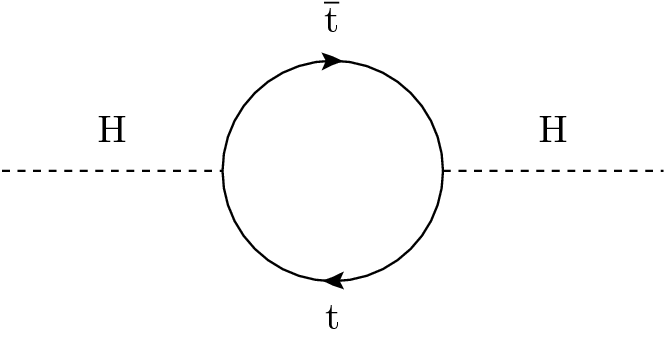
\includegraphics[width=0.7\textwidth]{higgs-loop.png}
\label{fig:susy:higgs-loop}
\caption{An example of a loop diagram which renormalizes the Higgs mass. Courtesy of PyFeyn.}
\end{figure}

%%%%%%%%%%%%%%%%  

Thus, the mass of the Higgs boson is not like that of other constants in the theory-- it is not arbitrary, like the masses of the quarks or leptons-- and the observed mass is substantially outside of the preferred range (at the Planck scale).  The SM's solution to this issue-- a precise cancelling of terms-- has an aesthetic penalty: there is no \textit{reason} for this cancellation in the SM, only blind luck. Physicists say that this kind of solution lacks \textit{naturalness}: there is no underlying symmetry or simplification to explain it, and only a complication of a very particular number.



\subsection{Unification}

Another aesthetic criticism of the SM lies in its separation of forces. The electroweak model is seen as particularly elegant because the electroweak symmetry, though broken at low energies by the Higgs mechanism, provides a unifying structure to two initially disparate forces (electomagnetism and the weak force). One natural question is whether some higher symmetry group unifies all the SM forces, and not just the electroweak. 


\subsection{Dark Matter}

One final motivation for the existence of physics beyond the SM is based on firm experimental ground and not just aesthetic preference: this is the presence of dark matter in the universe. 

\section{Supersymmetry: The Solution?}

These three shortcomings of the SM motivate the need for new theories-- but it turns out that one particularly interesting theory solves all three problems at once. This theory, called \textit{supersymmetry}, solves the problems of the SM in a very elegant way, by introducing a new symmetry between bosons and fermions. 

\subsection{Developing SUSY} 


Constructing such a theory with new particles requires constructing a Lagrangian that contains them; an unbroken supersymmetric theory is most naturally written in terms of supermultiplets to maintain the explicit supersymmetry. In particular, the requirement that members of supermultiplets have different spins means that the generators of the transformations ($\epsilon$) are fermionic fields (composed of Grassman numbers). The commutator of two supersymmetric fields introduces a $\gamma^\mu$ term, which must be contracted with a $\partial_\mu$ to create Lorentz invariant terms:
\begin{align}
  [\delta(\epsilon_1),\delta(\epsilon_2)] = \frac{1}{2} \left( \overline{\epsilon_2} \gamma^\mu \epsilon_1\right)\partial_\mu
\end{align}
These generators create the broken SU(3)$\times$ SU(2) $\times$ U(1) gauge symmetry that defines the MSSM. There is another type of well-motivated symmetry we would like to preserve: \cite[p.~231]{Jungman} $R$ parity is defined as $R = (-1)^{3(B-L)+2S}$ where $B$ is baryon number, $L$ is lepton number, and $S$ is spin. Thus, $R = 1$ for SM particles and $R = -1$ for SUSY particles. The preservation of $R$ parity is critical to generating a SUSY WIMP candidate: if $R$ was not preserved, SUSY particles with masses $\mathcal{O}(\mathrm{GeV})$ could decay to SM particles, and no stable LSP would exist. $R$ parity conservation also forbids terms that lead to baryon and lepton number violation which are strongly experimentally constrained. The Lagrangian for the MSSM that we are considering, in the spirit of the simplest, most minimal theory, will thus require invariance under SUSY transformations, R parity, and renormalizability for all terms. \cite[p.~231]{Jungman} 

%cite georgi at some point? why not

For completeness, let us now write out an example of a superfield which enters the Lagrangian. The relationships between terms are given as polynomials in abstract spinor symbols $\theta_\alpha$ and $\overline{\theta}_{\dot{\alpha}}$ which represent the superspace coordinates. A generic superfield will thus be of the form: \cite[p.~342]{Jungman}
\begin{align}
  \Phi(x, \theta_\alpha, \overline{\theta}_{\dot{\alpha}}) &= f(x) + \theta_\alpha \psi^\alpha(x) + \overline{\theta}_{\dot{\alpha}} \chi^{\dot{\alpha}} + \theta_\alpha \theta^\alpha m(x) + \overline{\theta}_{\dot{\alpha}} \overline{\theta}^{\dot{\alpha}} + \theta_\alpha \s^{\mu \alpha \dot{\alpha}} \overline{\theta}_{\dot{\alpha}} v_\mu(x) \nonumber\\
  &\quad + \theta_\alpha \theta^\alpha \overline{\theta}_{\dot{\alpha}} \overline{X}^{\dot{\alpha}}(x) + \overline{\theta}_{\dot{\alpha}} \overline{\theta}^{\dot{\alpha}} \theta_\alpha \phi^\alpha (x) + \theta_\alpha \theta^\alpha \overline{\theta}_{\dot{\alpha}} \overline{\theta}^{\dot{\alpha}}\mathrm{d}(x)
\end{align}
As expected, we have spinor, vector, and scalar fields. Some of these will be non-dynamical and can be integrated out using the equations of motion; the remaining terms will be the SM particles and their SUSY partners. Using the integration definitions for the Grassman-valued $\theta$'s, and putting together standard renormalizable action terms, we have a generic action of: \cite[p.~343]{Jungman}
\begin{align}
  S = \int d^4 x\left[ \int d^2\theta d^2 \theta \Phi^\dagger \Phi + \int d^2\theta \left( \lambda \Phi + m \Phi \Phi + \kappa \Phi \Phi \Phi \right) \right]
\end{align}
The first term is the standard kinetic term; the second term is the superpotential. The question now is what superfields to actually include. Inspired by the Standard Model choices, we want to include quark/lepton superfields of the form $\hat{L}_{Li}$, $\hat{c}_{Ri}$, $\hat{Q}_{Li}$, $\hat{d}_{Ri}$, $\hat{u}_{Ri}$, where $i$ is a generational index and $L$ or $R$ indicate handedness. Additionally, two Higgs superfields are required, $\hat{H}_1$ and $\hat{H}_2$, to give mass to all particles. \footnote{One Higgs is not sufficient, as traditionally down-type quarks acquire mass from a $H^c = i \tau_2 H^*$ type interaction, but the $H^*$ field is allowed in the supersymmetric Lagrangian. Another Higgs particle is thus required to give mass to down-type quarks and the other particles that $H^c$ would normally have interacted with.} Note that hats indicate superfields, as opposed to normal fields. Additionally, we should add on the vector superfields that of the U(1)$_Y\times$SU(2)$_W\times$SU(3)$_c$ gauge symmetry: $\hat{B}$, $\hat{W}^a$, and $\hat{G}^a$. \cite[p.~344]{Jungman}

With these fields, and the general form of an acceptable action written above, we can assemble the supersymmetric Lagrangian:
\begin{align}
  \mathcal{L}_s = \mathcal{L}_\mathrm{vector~kinetic} + \mathcal{L}_\mathrm{minimial~coupling} + \int d^2\theta \left( -\mu \hat{H}_1 \hat{H}_2 + \hat{H}_1 h_c^{ij}\hat{L}_{Li} \hat{e}_{Rj} + \hat{H}_1 h^{ij}_d \hat{Q}_{Li} \hat{d}_{Rj} - \hat{H}_2 h^{ij}_u \hat{Q}_{Li} \hat{u}_{Rj} \right)
\end{align}
where the term being integrated over $\theta$ is the superpotential $\mathcal{W}$. The $h$ matrices here are Yukawa-type coupling matrices derived from the mass matrices $M_c$, $M_u$, and $M_d$ in the standard configuration:
\begin{align}
  h_e = \frac{g}{\sqrt{2} m_w \cos{\beta}}M_e\quad \quad h_d = \frac{g}{\sqrt{2} m_w \cos{\beta}}M_d \quad \quad h_u = \frac{g}{\sqrt{2} m_w \sin{\beta}}M_u
\end{align}
where $\tan{\beta}$ is the ratio of vevs for the two Higgs fields. This theory is now manifestly supersymmetric, as it contains only superfields invariant under supersymmetry. Of course, it is understood that at energies below a scale $E_{sb}$, spontaneous symmetry breaking occurs and supersymmetry is broken. But, it is important that it breaks in such a way that the softened ultraviolet behavior of the radiative corrections is preserved. In particular, the most general gauge-invariant terms that break supersymmetry but respect our other conditions are, following Girardello and Grisaru: \cite[p.~346]{Jungman}
\begin{align}
  \mathcal{L}_\mathrm{soft} = &-m_1^2 |H_1|^2 - m_2^2 |H_2|^2 - m_{12}^2 \left( H_1 H_2 + H_1^* H_2^* \right) - \tilde{Q}_{Li}^\dagger M_{\tilde{Q} ij}^2 \tilde{Q}_{Lj} - \tilde{u}^\dagger_{Ri} M^2_{\tilde{u} i j} \tilde{u}_{Rj}\nonumber\\
  &-\tilde{d}_{Ri}^\dagger M^2_{\tilde{d} i j} \tilde{d}_{Rj} -\hat{L}^\dagger_{Li} M^2_{\tilde{L} ij} \tilde{L}_{Lj} - \tilde{e}^*_{Ri} M^2_{\tilde{e} ij} \tilde{e}_{Rj} + H_2 \tilde{Q}_{Li}(h_u A_u)_{ij} \tilde{u}_{Rj} -H_1 \tilde{Q}_{Li} (h_d A_d)_{ij} \tilde{d}_{Rj}\nonumber\\
  &-H_1 \tilde{L}_{Li} (h_e A_e)_{ij} \tilde{e}_{Rj} - \frac{1}{2} \left[ M_1 \overline{\tilde{B}} \tilde{B} + M_2 \overline{\tilde{W}}^a \overline{W}^a + M_3 \overline{\tilde{G}}^a \tilde{G}^a \right]
\end{align}
where $A$ terms are mass matrices in flavor space, and the rest of the definitions are relatively clear. The fields here are no longer superfields, and the $\sim$ indicate superpartners of Standard Model fields. Combined with $\mathcal{L}_s$, this gives a full description of the particles and fields of a broken supersymmetric theory, but the superfields from $\mathcal{L}_s$ remain. Since we have already broken supersymmetry, we may as well integrate out the auxiliary fields and break their manifest symmetry.

From astrophysics observations, we know that a candidate WIMP must be heavy and neutral, so we are interested in the SUSY particles which fit this criterea. In particular, what matters to us is the particular linear combination of $\tilde{B}$, $\tilde{W}^3$, $\tilde{H}_1^0$, and $\tilde{H}_2^0$. The superpotential introduces quadratic couplings between the these four fields when the supersymmetry is broken and after the Higgs particles have acquired a vev and spontaneously broken the remaining symmetry. In particular, the couplings are defined by the mass matrix:
\begin{align}
  M_\mathrm{neut}=
\left(
\begin{array}{cccc}
 M_1 & 0 & -c_{\beta } m_z s_w &
   m_z s_{\beta } s_w \\
 0 & M_2 & c_{\beta } c_w m_z &
   -c_w m_z s_{\beta } \\
 -c_{\beta } m_z s_w & c_{\beta }
   c_w m_z & 0 & -\mu  \\
 m_z s_{\beta } s_w & -c_w m_z
   s_{\beta } & -\mu  & 0
\end{array}
\right)  \label{eqn:massx}
\end{align}
This matrix is in the $\tilde{B}-\tilde{W}^3-\tilde{H}_1^0-\tilde{H}_2^0$ basis, and diagonalized by a transformation: $M_\mathrm{neut}^\mathrm{diag} = N^\dagger M_\mathrm{neut} N$, where we expect $N$ to appear as a mixing matrix in neutralino interaction terms. From the diagonalization of this matrix, 4 mass eigenstates appear, labelled $\chi_m^0$ with $m\in\{1,2,3,4\}$ \cite[p.~349]{Jungman}. Heavy neutralinos will decay down the spectrum to the lightest.

However, it is not immediately clear what makes the $\chi$ a good candidate to be the LSP, as other superparticles could be lighter.  But the Higgsinos have Yukawa couplings to other particles, and in particular the large contributions of top loops lead Yukawa couplings to run negative in low energies \cite[p.~80]{Martin1997}. While the exact values of the runnings are of course very model dependent, Figure~\ref{fig:mass-run} gives an example of this sort of running \cite[p.~80]{Martin1997}. The dominant effect on $M_1$ is indeed the top-Yukawa coupling which pulls down the mass below others, whereas SU(3) couplings pull the mass of squarks much higher, for example \cite[p.~81]{Martin1997}.



Writing out the mixing parameters explicitly, we thus have:
\begin{align}
  \chi = N_{10}^* \tilde{B} + N_{20}^* \tilde{W}^3 + N_{30}^* \tilde{H}_1^0 + N_{40}^* \tilde{H}_2^0
\end{align}
where $N$ is the neutralino mixing matrix which arises from the diagonalization of the mass matrix in eqn. \ref{eqn:massx}. 

We have shown, then, that $MSSM$ produces a wide variety of new particles when we write down an initial unbroken Lagrangian using superfields that must be invariant under SUSY transformations. Soft, explicit breaking of the supersymmetry introduces additional couplings; combined with the couplings in the superfields themselves, we generate a mass matrix $M_\mathrm{neut}$ which couples the Higgsinos, Bino, and Wino fields. Diagonalizing this matrix leads to new mass eigenstates, the neutralinos $\chi$. The lightest of these is a good candidate to be the LSP, as RG running of masses makes most other particles much heavier at energies below the supersymmetry breaking scale.

\subsection{Fixing Naturalness}

\subsection{Coupling Unification}

\subsection{Dark Matter}

\section{The Status of SUSY after LHC Run 1}


\section{$R$-Parity, and How to Violate It}

		 ...